\chapter{MULTIPLY-ACCUMULATOR}
\label{chp:mac}
\begin{figure}
    \centering
\begin{tikzpicture}[scale=1]
\clip (-5,-2.5) rectangle (5,2.5);
\node at (0,0) [draw, rectangle, minimum height=4cm, minimum width=8cm, label={[label distance=-.6cm,xshift=-2cm]90:Multiply-Accumulator}](acc){};
\node at (acc) [draw, rectangle, xshift=3cm, yshift=0cm, minimum height=1cm, minimum width=2cm](add){Adder};
\node at (acc) [draw, rectangle, xshift=.3cm, yshift=0cm, minimum height=1cm, minimum width=0](int){\shortstack{Intermediator}};
\node at (acc) [draw, rectangle, xshift=-3cm, yshift=0cm, minimum height=1cm, minimum width=2cm](mult){\shortstack{Multiplier}};

\path [draw, thick, >=stealth',->] (-5,.3) --node[ fill=white, inner sep=1pt]{val} (-4,.3) ;
\path [draw, thick, >=stealth',->] (-5,0) --node[ fill=white, inner sep=1pt]{val} (-4,0) ;
\path [draw, thick, >=stealth',->] (-5,-.3) --node[ fill=white, inner sep=1pt]{row} (-4,-.3);

\path [draw, thick, >=stealth',->] (-2,0) --node[ fill=white, inner sep=1pt]{val} (-1,0);
\path [draw, thick, >=stealth',->] (-2,-.3) --node[ fill=white, inner sep=1pt]{row} (-1,-.3) ;

\path [draw, thick, >=stealth',->] (.4,.5)  arc(160:20:1.2);
\node at (1.5,1.2)[fill=white, inner sep=1pt]{row};

\path [draw, thick, >=stealth',->] (.1,.5)  arc(163:17:1.5);
\node at (1.5,1.5)[fill=white, inner sep=1pt]{val};

\path [draw, thick, >=stealth',->] (-.2,.5)  arc(166:14:1.8);
\node at (1.5,1.8)[fill=white, inner sep=1pt]{val};

\path [draw, thick, >=stealth',->] (2.6,-.5)  arc(-20:-160:1.2);
\node at (1.5,-1.2)[fill=white, inner sep=1pt]{row};

\path [draw, thick, >=stealth',->] (2.9,-.5)  arc(-17:-163:1.5);
\node at (1.5,-1.5)[fill=white, inner sep=1pt]{val};

\path [draw, thick, >=stealth',->] (-.5,-.5) --node[sloped, fill=white, inner sep=1pt]{val} (-.5,-2.5);
\end{tikzpicture} %

\caption[Multiply-accumulator]{The no-stall multiply-accumulator block handles multiple intermediate values at a time. This allows multiple intermediate values in the adder pipeline.}
\label{fig:mac}
\end{figure}
A high throughput SpMV implementation relies on designing a no-stall multiply accumulator (MAC). An inefficient engine stalls when a matrix and its associated vector value arrives every or nearly every clock cycle. The long latency of floating point addition makes this complicated. To solve this, our approach works on multiple intermediate $y$ vector values and does the additions out of order (\figurename~\ref{fig:mac}). So, $y[i]$ can still be accumulating while processing $y[i+1]$. For an example of out of order addition, when computing $1+2+3+4$ the MAC does $(1+2)+(3+4)$. This removes the data dependency of adding $1$ and $2$ before processing $3$. CPUs and GPUs compute floating point addition in order (eg. $\left((1+2)+3\right)+4$). This means results may differ slightly, because changing the order of floating point addition can change the result [\cite{prelim:goldberg}].\\
\indent In $R^3$ [\cite{prelim:townsend}] we designed a block called an Intermediator capable of storing 32 intermediate $y$ vector values. In our next design we intend to expand this to 1024 (the depth of one dual port RAM blocks in most Xilinx chips). Both designs have an interesting side effect that the allow the matrix to be traversed in a loosely row major traversal and the MAC still works correctly. The step to from 32 to 1024 intermediate values allows more freedom in the traversal. The rest of the chapter discusses the new design. The matrix elements in one set of 512 rows can be traversed in any way just as long as all the elements are traversed before going to the next 512 rows. Later in chapter 5 we discuss traversals that abide by this rule and allow for easy reuse of $x$ vector values.
\section{Intermediator}
\label{sec:intermediator}
The Intermediator (Figure \ref{intermediatorEx}) takes in two values, one from the multiplier's result and one from the adder's result and outputs a pair of values to be added together. The dual-port RAM block (the middle block in Figure \ref{intermediatorEx}) stores intermediate values until an element in the same row appears. \par
For large matrices, the RAM blocks cannot store the entire intermediate $y$ vector. Also the control logic needs to remember the state of each slot in RAM (vacant or occupied). Remembering the state of each RAM location and updating that state requires a dual-port RAM with zero clock cycle latency. This type of RAM does not exist in the FPGA fabric. In $R^3$, we approach this problem by using FPGA logic which limits the number of active intermediate values to 32. In our new design we will use distributed RAM with a width of 1 bit to keep track of the state of each slot (discussed later in Section \ref{sec:dualmemory}). \par
The cells in the intermediator have four states which we call the red, yellow, green and white states, in addition to the vacant/occupied state. The memory is split in 2, an upper and lower section. Once the accumulation starts, one of these sections will be in the red active state. Once the incoming values move to the next 512 row section of the matrix this section transitions to the yellow fading state, and the new section of the memory is now in the red active state. Recall our traversal rule is that each 512 rows must be traversed before proceeding to the next 512 rows. The yellow fading state exists because values are still being accumulated in the previously active memory. The memory will always be accumulated within 80 clock cycles. At that point the faded state transitions to the green ``read to store" state. Once the values have been sent out to be stored the memory transitions to the white idle state.
\par To understand why at most 80 cycle cycles are needed to ensure the accumulation has finished after no new values arrive from the multiplier, let us look at the worst case operation. Only inputs from the adder correspond with to the elements in the fading window and the multiplier should not output values belong to the fading window. So, the theoretical worst case occurs with a full adder pipeline and each value corresponds to the same row. Every 16 cycles (the adder pipeline length) the number of elements with the same row in the pipeline cuts in half. Therefore, the worst case would take 80 ($(\log_2(16) + 1) \times 16$) clock cycles to guarantee that no fading elements get sent to the adder and the fading window only has final $y$ vector values. The worst case would also advance the window in 512 clock cycles (1 element per row in the matrix for those 512 rows corresponding to the active window). It also takes 512 cycles to store the green ``ready to store" elements. So in theory the MAC could stall, but in practice this never happens.
\par Many cases occur when accumulating values in multiple rows and the Intermediator handles each case properly:
\\\indent Case 1: (Figure \ref{cycle7}) The trivial case, no valid input arrives. If the ``to result" block has values, it outputs a pair of values to the adder. An overflow FIFO (explained in case 6) outputs a value if it has values.
\\\indent Case 2: (Figure \ref{cycle4}) Only one value arrives and the row corresponds to a vacant cell. The value goes into the vacant cell. If the ``to result" window has values, it outputs a result, and if the overflow FIFO has values it outputs a set to the adder.
\\\indent Case 3: (Figure \ref{cycle1}) Similar to case 2 except with an occupied cell. It retrieves the value in the Intermediator cell and goes to the adder with the input value. The state of the cell gets updated to vacant.
\\\indent Case 4: (Figure \ref{cycle2}, \ref{cycle8}) Both values have row indexes that correspond to vacant cells in the RAM block. Both values get stored in the RAM block and both cells switch to occupied. If the overflow FIFO has values it sends one set of values to the output. 
\\\indent Case 5: (Figure \ref{cycle6}) One value has a row index corresponding to a vacant cell, and the other to an occupied cell. The first value goes in the vacant cell and the value in the occupied cell goes to the adder with the second value. 
\\\indent Case 6: (Figure \ref{cycle3}) Both values have row indexes that correspond to occupied cells in the RAM. One input value and its corresponding Intermediator cell's value go to the output. The output can only handle one output pair at a time, so the other input value and its corresponding Intermediator cell's value go to the overflow FIFO.
\\\indent Case 7: (Figure \ref{cycle5}) The values have identical row indices. In this case, the values go through the pipeline and do not touch the Intermediator cells. They simply pass through to the adder.\\
%
\begin{figure*}
\begin{multicols}{3}
\begin{subfigure}{\linewidth}
\begin{tikzpicture}
\node (a) {Input};
\node (b)[below=of a] {Result};
\node (c)[right=of a,xshift=-.6cm,yshift=.2cm] {RAM};
\draw (c) +(-.5,0.2) rectangle ++(.5,-2.2);
\node (d)[xshift=-.7cm,yshift=-.5cm,right=of c, draw, minimum width=1.5cm, minimum height=.5cm, label=above:FIFO]{};
\node (e1) at ([xshift=-.6cm]d) [draw, rectangle, minimum height=.5cm, minimum width=.3cm,pattern=north east lines]{};
\node (e)[below=of d, yshift=.3cm]{Adder};
%\node (f) at ([yshift=-2cm]c) [draw,minimum width=1.5cm]{};
%\coordinate (s16) at ($ (c) - (.5,0) $);
%\draw (s16) rectangle ++(.5,.5);
\foreach [count=\i] \y in {-1.85,-1.6,...,-.1}{
	\node (n\i) at ([xshift=-0cm,yshift=-.2cm+\y cm]c) [minimum height=.25cm, minimum width=1cm]{};
}
%\node (active) at ([xshift=.7cm,yshift=0cm]n5) [draw,fill=red!30,rectangle,minimum width=1cm,minimum height=.25cm]{};
\draw[pattern=north east lines,preaction={fill,red}] ([xshift=-.5cm,yshift=-.125cm]n5) rectangle ([xshift=.5cm,yshift=.125cm]n6);
\draw[preaction={fill,red}] ([xshift=-.5cm,yshift=-.125cm]n7) rectangle ([xshift=.5cm,yshift=.125cm]n8);
\draw[pattern=north east lines,preaction={fill,green}] ([xshift=-.5cm,yshift=-.125cm]n1) rectangle ([xshift=.5cm,yshift=.125cm]n4);
%\draw[pattern=north east lines,preaction={fill,green}] ([xshift=-.5cm,yshift=-.125cm]n2) rectangle ([xshift=.5cm,yshift=.125cm]n2);
\foreach [count=\i] \y in {-1.85,-1.6,...,-.1}{
    \FPeval{\n}{round(\i-1:0)}
	\node (m\i) at ([xshift=-0.7cm,yshift=-.2cm+\y cm]c) []{\scriptsize \n};
}

\path [draw, thick, >=stealth',->](a) to [bend right=20] (e);

\path [draw, thick, >=stealth',->](n1.west) to [bend right=0] (b);
\draw [->,thick, >=stealth'] (n6.east) to [bend left=10] (e);
%\tikzstyle{line} = [draw, thick, -latex' ,shorten >=2pt];
\end{tikzpicture}
\caption{First clock cycle, 1 pair of values get sent to the adder.}
\label{cycle1}
\end{subfigure}

\begin{subfigure}{\linewidth}
\begin{tikzpicture}
\node (a) {Input};
\node (b)[below=of a] {Result};
\node (c)[right=of a,xshift=-.6cm,yshift=.2cm] {RAM};
\draw (c) +(-.5,0.2) rectangle ++(.5,-2.2);
\node (d)[xshift=-.7cm,yshift=-.5cm,right=of c, draw, minimum width=1.5cm, minimum height=.5cm, label=above:FIFO]{};
\node (e1) at ([xshift=-.6cm]d) [draw, rectangle, minimum height=.5cm, minimum width=.3cm,pattern=north east lines]{};
\node (e)[below=of d, yshift=.3cm]{Adder};
%\node (f) at ([yshift=-2cm]c) [draw,minimum width=1.5cm]{};
%\coordinate (s16) at ($ (c) - (.5,0) $);
%\draw (s16) rectangle ++(.5,.5);
\foreach [count=\i] \y in {-1.85,-1.6,...,-.1}{
	\node (n\i) at ([xshift=-0cm,yshift=-.2cm+\y cm]c) [minimum height=.25cm, minimum width=1cm]{};
}
%\node (active) at ([xshift=.7cm,yshift=0cm]n5) [draw,fill=red!30,rectangle,minimum width=1cm,minimum height=.25cm]{};
\draw[fill=red] ([xshift=-.5cm,yshift=-.125cm]n5) rectangle ([xshift=.5cm,yshift=.125cm]n8);
\draw[pattern=north east lines] ([xshift=-.5cm,yshift=-.125cm]n5) rectangle ([xshift=.5cm,yshift=.125cm]n5);
\draw[pattern=north east lines,preaction={fill,green}] ([xshift=-.5cm,yshift=-.125cm]n2) rectangle ([xshift=.5cm,yshift=.125cm]n4);
\foreach [count=\i] \y in {-1.85,-1.6,...,-.1}{
    \FPeval{\n}{round(\i-1:0)}
	\node (m\i) at ([xshift=-0.7cm,yshift=-.2cm+\y cm]c) []{\scriptsize \n};
}

\path [draw, thick, >=stealth',->](a) to [bend right=20] (n6.west);
\path [draw, thick, >=stealth',->](a) to [bend right=10] (n7.west);
%\edge [draw, thick, ->, bend right] (e2.south) -- (e);
\draw [->,thick, >=stealth'] (e1) to [bend right=10] (e);
%\tikzstyle{line} = [draw, thick, -latex' ,shorten >=2pt];
\end{tikzpicture}
\caption{Second clock cycle, 2 values gets stored in the RAM.}
\label{cycle2}
\end{subfigure}

\begin{subfigure}{\linewidth}
\centering
\begin{tikzpicture}
\node (a) {Input};
\node (b)[below=of a] {Result};
\node (c)[right=of a,xshift=-.6cm,yshift=.2cm] {RAM};
\draw (c) +(-.5,0.2) rectangle ++(.5,-2.2);
\node (d)[xshift=-.7cm,yshift=-.5cm,right=of c, draw, minimum width=1.5cm, minimum height=.5cm, label=above:FIFO]{};
\node (e)[below=of d, yshift=.3cm]{Adder};
%\node (f) at ([yshift=-2cm]c) [draw,minimum width=1.5cm]{};
%\coordinate (s16) at ($ (c) - (.5,0) $);
%\draw (s16) rectangle ++(.5,.5);
\foreach [count=\i] \y in {-1.85,-1.6,...,-.1}{
	\node (n\i) at ([xshift=-0cm,yshift=-.2cm+\y cm]c) [minimum height=.25cm, minimum width=1cm]{};
}
%\node (active) at ([xshift=.7cm,yshift=0cm]n5) [draw,fill=red!30,rectangle,minimum width=1cm,minimum height=.25cm]{};
\draw[fill=red] ([xshift=-.5cm,yshift=-.125cm]n5) rectangle ([xshift=.5cm,yshift=.125cm]n8);
\draw[pattern=north east lines] ([xshift=-.5cm,yshift=-.125cm]n5) rectangle ([xshift=.5cm,yshift=.125cm]n7);
\draw[pattern=north east lines,preaction={fill,green}] ([xshift=-.5cm,yshift=-.125cm]n2) rectangle ([xshift=.5cm,yshift=.125cm]n4);
\foreach [count=\i] \y in {-1.85,-1.6,...,-.1}{
    \FPeval{\n}{round(\i-1:0)}
	\node (m\i) at ([xshift=-0.7cm,yshift=-.2cm+\y cm]c) []{\scriptsize \n};
}

\path [draw, thick, >=stealth',->](a) to [bend left=10] (d);
\path [draw, thick, >=stealth',->](n7.east) to [bend left=1] (d);
\path [draw, thick, >=stealth',->](a) to [bend right=0] (e);
\path [draw, thick, >=stealth',->](n6.east) to [bend left=30](e);
\end{tikzpicture}
\caption{Third clock cycle, the 2 inputs correspond to occupied cells in the RAM block.}
\label{cycle3}
\end{subfigure}

\end{multicols}
%
\begin{multicols}{3}
\begin{subfigure}{\linewidth}
\begin{tikzpicture}
\node (a) {Input};
\node (b)[below=of a] {Result};
\node (c)[right=of a,xshift=-.6cm,yshift=.2cm] {RAM};
\draw (c) +(-.5,0.2) rectangle ++(.5,-2.2);
\node (d)[xshift=-.7cm,yshift=-.5cm,right=of c, draw, minimum width=1.5cm, minimum height=.5cm, label=above:FIFO]{};
\node (e1) at ([xshift=-.6cm]d) [draw, rectangle, minimum height=.5cm, minimum width=.3cm,pattern=north east lines]{};
\node (e)[below=of d, yshift=.3cm]{Adder};
%\node (f) at ([yshift=-2cm]c) [draw,minimum width=1.5cm]{};
%\coordinate (s16) at ($ (c) - (.5,0) $);
%\draw (s16) rectangle ++(.5,.5);
\foreach [count=\i] \y in {-1.85,-1.6,...,-.1}{
	\node (n\i) at ([xshift=-0cm,yshift=-.2cm+\y cm]c) [minimum height=.25cm, minimum width=1cm]{};
}
%\node (active) at ([xshift=.7cm,yshift=0cm]n5) [draw,fill=red!30,rectangle,minimum width=1cm,minimum height=.25cm]{};
\draw[fill=red] ([xshift=-.5cm,yshift=-.125cm]n5) rectangle ([xshift=.5cm,yshift=.125cm]n8);
\draw[pattern=north east lines] ([xshift=-.5cm,yshift=-.125cm]n5) rectangle ([xshift=.5cm,yshift=.125cm]n5);
\draw[pattern=north east lines,preaction={fill,green}] ([xshift=-.5cm,yshift=-.125cm]n2) rectangle ([xshift=.5cm,yshift=.125cm]n4);
\foreach [count=\i] \y in {-1.85,-1.6,...,-.1}{
    \FPeval{\n}{round(\i-1:0)}
	\node (m\i) at ([xshift=-0.7cm,yshift=-.2cm+\y cm]c) []{\scriptsize \n};
}

\path [draw, thick, >=stealth',->](a) to [bend right=10] (n7.west);
\path [draw, thick, >=stealth',->](n2.west) to (b);
\draw [->,thick, >=stealth'] (e1) to [bend right=10] (e);
%\tikzstyle{line} = [draw, thick, -latex' ,shorten >=2pt];
\end{tikzpicture}
\caption{Fourth clock cycle, 1 value gets stored in RAM.}
\label{cycle4}
\end{subfigure}
\begin{subfigure}{\linewidth}
\centering
\begin{tikzpicture}
\node (a) {Input};
\node (b)[below=of a] {Result};
\node (c)[right=of a,xshift=-.6cm,yshift=.2cm] {RAM};
\draw (c) +(-.5,0.2) rectangle ++(.5,-2.2);
\node (d)[xshift=-.7cm,yshift=-.5cm,right=of c, draw, minimum width=1.5cm, minimum height=.5cm, label=above:FIFO]{};
\node (e)[below=of d, yshift=.3cm]{Adder};
%\node (f) at ([yshift=-2cm]c) [draw,minimum width=1.5cm]{};
%\coordinate (s16) at ($ (c) - (.5,0) $);
%\draw (s16) rectangle ++(.5,.5);
\foreach [count=\i] \y in {-1.85,-1.6,...,-.1}{
	\node (n\i) at ([xshift=-0cm,yshift=-.2cm+\y cm]c) [minimum height=.25cm, minimum width=1cm]{};
}
%\node (active) at ([xshift=.7cm,yshift=0cm]n5) [draw,fill=red!30,rectangle,minimum width=1cm,minimum height=.25cm]{};
\draw[fill=red] ([xshift=-.5cm,yshift=-.125cm]n5) rectangle ([xshift=.5cm,yshift=.125cm]n8);
\draw[pattern=north east lines] ([xshift=-.5cm,yshift=-.125cm]n5) rectangle ([xshift=.5cm,yshift=.125cm]n5);
\draw[pattern=north east lines] ([xshift=-.5cm,yshift=-.125cm]n7) rectangle ([xshift=.5cm,yshift=.125cm]n7);
\draw[pattern=north east lines,preaction={fill,green}] ([xshift=-.5cm,yshift=-.125cm]n3) rectangle ([xshift=.5cm,yshift=.125cm]n4);
\foreach [count=\i] \y in {-1.85,-1.6,...,-.1}{
    \FPeval{\n}{round(\i-1:0)}
	\node (m\i) at ([xshift=-0.7cm,yshift=-.2cm+\y cm]c) []{\scriptsize \n};
}

\path [draw, thick, >=stealth',->](a) to [bend left=10] (e);
\path [draw, thick, >=stealth',->](a) to [bend right=10] (e);
\path [draw, thick, >=stealth',->](n3.west) to [bend right=5] (b);
%\edge [draw, thick, ->, bend right] (e2.south) -- (e);
%\tikzstyle{line} = [draw, thick, -latex' ,shorten >=2pt];
\end{tikzpicture}
\caption{Fifth clock cycle, the row indexes of the 2 inputs equal each other.}
\label{cycle5}
\end{subfigure}

\begin{subfigure}{\linewidth}
\begin{tikzpicture}
\node (a) {Input};
\node (b)[below=of a] {Result};
\node (c)[right=of a,xshift=-.6cm,yshift=.2cm] {RAM};
\draw (c) +(-.5,0.2) rectangle ++(.5,-2.2);
\node (d)[xshift=-.7cm,yshift=-.5cm,right=of c, draw, minimum width=1.5cm, minimum height=.5cm, label=above:FIFO]{};
\node (e)[below=of d, yshift=.3cm]{Adder};
%\node (f) at ([yshift=-2cm]c) [draw,minimum width=1.5cm]{};
%\coordinate (s16) at ($ (c) - (.5,0) $);
%\draw (s16) rectangle ++(.5,.5);
\foreach [count=\i] \y in {-1.85,-1.6,...,-.1}{
	\node (n\i) at ([xshift=-0cm,yshift=-.2cm+\y cm]c) [minimum height=.25cm, minimum width=1cm]{};
}
%\node (active) at ([xshift=.7cm,yshift=0cm]n5) [draw,fill=red!30,rectangle,minimum width=1cm,minimum height=.25cm]{};
\draw[fill=red] ([xshift=-.5cm,yshift=-.125cm]n5) rectangle ([xshift=.5cm,yshift=.125cm]n8);
\draw[pattern=north east lines] ([xshift=-.5cm,yshift=-.125cm]n7) rectangle ([xshift=.5cm,yshift=.125cm]n7);
\draw[pattern=north east lines,preaction={fill,green}] ([xshift=-.5cm,yshift=-.125cm]n4) rectangle ([xshift=.5cm,yshift=.125cm]n4);
\draw[pattern=north east lines] ([xshift=-.5cm,yshift=-.125cm]n5) rectangle ([xshift=.5cm,yshift=.125cm]n5);
\foreach [count=\i] \y in {-1.85,-1.6,...,-.1}{
    \FPeval{\n}{round(\i-1:0)}
	\node (m\i) at ([xshift=-0.7cm,yshift=-.2cm+\y cm]c) []{\scriptsize \n};
}

\path [draw, thick, >=stealth',->](a) to [bend right=20] (n6.west);
\path [draw, thick, >=stealth',->](a) to [bend left=5] (e);
\path [draw, thick, >=stealth',->](n7.east) to [bend left=20] (e);
\end{tikzpicture}
\caption{Sixth clock cycle, 1 pair of values get sent to the adder, and 1 element gets stored in RAM.}
\label{cycle6}
\end{subfigure}

\end{multicols}
%
\begin{multicols}{3}
\begin{subfigure}{\linewidth}
\centering
\begin{tikzpicture}
\node (a) {Input};
\node (b)[below=of a] {Result};
\node (c)[right=of a,xshift=-.6cm,yshift=.2cm] {RAM};
\draw (c) +(-.5,0.2) rectangle ++(.5,-2.2);
\node (d)[xshift=-.7cm,yshift=-.5cm,right=of c, draw, minimum width=1.5cm, minimum height=.5cm, label=above:FIFO]{};
\node (e)[below=of d, yshift=.3cm]{Adder};
%\node (f) at ([yshift=-2cm]c) [draw,minimum width=1.5cm]{};
%\coordinate (s16) at ($ (c) - (.5,0) $);
%\draw (s16) rectangle ++(.5,.5);
\foreach [count=\i] \y in {-1.85,-1.6,...,-.1}{
	\node (n\i) at ([xshift=-0cm,yshift=-.2cm+\y cm]c) [minimum height=.25cm, minimum width=1cm]{};
}
%\node (active) at ([xshift=.7cm,yshift=0cm]n5) [draw,fill=red!30,rectangle,minimum width=1cm,minimum height=.25cm]{};
\draw[fill=red] ([xshift=-.5cm,yshift=-.125cm]n5) rectangle ([xshift=.5cm,yshift=.125cm]n8);
\draw[pattern=north east lines,preaction={fill,green}] ([xshift=-.5cm,yshift=-.125cm]n4) rectangle ([xshift=.5cm,yshift=.125cm]n4);
\draw[pattern=north east lines] ([xshift=-.5cm,yshift=-.125cm]n5) rectangle ([xshift=.5cm,yshift=.125cm]n6);
\foreach [count=\i] \y in {-1.85,-1.6,...,-.1}{
    \FPeval{\n}{round(\i-1:0)}
	\node (m\i) at ([xshift=-0.7cm,yshift=-.2cm+\y cm]c) []{\scriptsize \n};
}
\path [draw, thick, >=stealth',->](n4.west) to [bend right=5] (b);
\end{tikzpicture}
\caption{Seventh clock cycle, no valid inputs.}
\label{cycle7}
\end{subfigure}

\begin{subfigure}{\linewidth}
\centering
\begin{tikzpicture}
\node (a) {Input};
\node (b)[below=of a] {Result};
\node (c)[right=of a,xshift=-.6cm,yshift=.2cm] {RAM};
\draw (c) +(-.5,0.2) rectangle ++(.5,-2.2);
\node (d)[xshift=-.7cm,yshift=-.5cm,right=of c, draw, minimum width=1.5cm, minimum height=.5cm, label=above:FIFO]{};
\node (e)[below=of d, yshift=.3cm]{Adder};
%\node (f) at ([yshift=-2cm]c) [draw,minimum width=1.5cm]{};
%\coordinate (s16) at ($ (c) - (.5,0) $);
%\draw (s16) rectangle ++(.5,.5);
\foreach [count=\i] \y in {-1.85,-1.6,...,-.1}{
	\node (n\i) at ([xshift=-0cm,yshift=-.2cm+\y cm]c) [minimum height=.25cm, minimum width=1cm]{};
}
%\node (active) at ([xshift=.7cm,yshift=0cm]n5) [draw,fill=red!30,rectangle,minimum width=1cm,minimum height=.25cm]{};
\draw[fill=red] ([xshift=-.5cm,yshift=-.125cm]n1) rectangle ([xshift=.5cm,yshift=.125cm]n4);
\draw[fill=yellow] ([xshift=-.5cm,yshift=-.125cm]n5) rectangle ([xshift=.5cm,yshift=.125cm]n8);
\draw[pattern=north east lines] ([xshift=-.5cm,yshift=-.125cm]n5) rectangle ([xshift=.5cm,yshift=.125cm]n6);
\foreach [count=\i] \y in {-1.85,-1.6,...,-.1}{
    \FPeval{\n}{round(\i-1:0)}
	\node (m\i) at ([xshift=-0.7cm,yshift=-.2cm+\y cm]c) []{\scriptsize \n};
}

\path [draw, thick, >=stealth',->](a) to [bend left=0] (n8.west);
\path [draw, thick, >=stealth',->](a) to [bend right=10] (n1.west);
\end{tikzpicture}
\caption{Eighth clock cycle, the 2 inputs correspond to vacant cells in the RAM block.}
\label{cycle8}
\end{subfigure}
\begin{subfigure}{\linewidth}
\centering
\begin{tikzpicture}
\node (a) {Input};
\node (b)[below=of a] {Result};
\node (c)[right=of a,xshift=-.6cm,yshift=.2cm] {RAM};
\draw (c) +(-.5,0.2) rectangle ++(.5,-2.2);
\node (d)[xshift=-.7cm,yshift=-.5cm,right=of c, draw, minimum width=1.5cm, minimum height=.5cm, label=above:FIFO]{};
\node (e)[below=of d, yshift=.3cm]{Adder};
%\node (f) at ([yshift=-2cm]c) [draw,minimum width=1.5cm]{};
%\coordinate (s16) at ($ (c) - (.5,0) $);
%\draw (s16) rectangle ++(.5,.5);
\foreach [count=\i] \y in {-1.85,-1.6,...,-.1}{
	\node (n\i) at ([xshift=-0cm,yshift=-.2cm+\y cm]c) [minimum height=.25cm, minimum width=1cm]{};
}
%\node (active) at ([xshift=.7cm,yshift=0cm]n5) [draw,fill=red!30,rectangle,minimum width=1cm,minimum height=.25cm]{};
\draw[fill=red] ([xshift=-.5cm,yshift=-.125cm]n1) rectangle ([xshift=.5cm,yshift=.125cm]n4);
\draw[fill=yellow] ([xshift=-.5cm,yshift=-.125cm]n5) rectangle ([xshift=.5cm,yshift=.125cm]n8);
\draw[pattern=north east lines] ([xshift=-.5cm,yshift=-.125cm]n5) rectangle ([xshift=.5cm,yshift=.125cm]n6);
\draw[pattern=north east lines] ([xshift=-.5cm,yshift=-.125cm]n8) rectangle ([xshift=.5cm,yshift=.125cm]n8);
\draw[pattern=north east lines] ([xshift=-.5cm,yshift=-.125cm]n1) rectangle ([xshift=.5cm,yshift=.125cm]n1);
\foreach [count=\i] \y in {-1.85,-1.6,...,-.1}{
    \FPeval{\n}{round(\i-1:0)}
	\node (m\i) at ([xshift=-0.7cm,yshift=-.2cm+\y cm]c) []{\scriptsize \n};
}

%\path [draw, thick, >=stealth',->](a) to [bend left=0] (n8.west);
%\path [draw, thick, >=stealth',->](a) to [bend right=10] (n1.west);
\end{tikzpicture}
\caption{Ninth clock cycle, the Intermediator has no inputs and nothing to send to the adder or final values to output.}
\label{cycle8}
\end{subfigure}
\end{multicols}

\caption[Intermediator]{This shows a simple example of the Intermediator running for 9 clock cycles. For demonstration, the size of the RAM is 8 instead of 1024.}
\label{intermediatorEx}
\end{figure*}
%
\indent
To help explain, consider a simpler case where the depth of the intermediator is 8 instead of 1024. Figure \ref{intermediatorEx} shows 8 clock cycles of operation. At every clock cycle up to 2 valid input values with corresponding row indexes arrive. For simplicity, we do not show the values being calculated in the figure.
%\section{Four RAM Blocks and Clever use of XOR}
\section{A Dual Port 1$\times$1024 RAM with Zero Clock Cycle Latency}
\label{sec:dualmemory}
We have not yet addressed the issue of keeping track of the vacant/occupied state of the cells in the Intermediator. To do this we need a dual port 1-bit RAM. In order to update the value in RAM in one clock cycle it must have no read latency. \par
We implement a special case of the memory developed in \cite{prelim:laforest2} to achieve this. This requires the use of pseudo dual port distributed RAMs. Before looking at the implementation let us look at the target behavior. During an intermidiator status request the bit of  the requested address will always flip. (Vacant cells become occupied and occupied cells become vacant.) This flip occurs the clock cycle after the status is reported.\par
FPGA vendors do not provide dual port distributed RAMs. Instead, they provide pseudo dual port distributed RAMs. That is RAMs with one read port and one write port. \par
With a clever arragement of 4 pseudo dual port RAMs we can emulate one dual port RAM. To begin with, arrange the RAMs in a $2\times 2$ grid. The write ports of the 2 RAMs in each row are connected together. The read ports of the 2 RAMs in each column are connected by an XOR gate. The address on Port 1 controls the address of the write port of the bottom row of RAMs. The address on Port 1 also controls the address of the read ports of the left column of RAMs. Similarly, the address on Port 2 controls the address of the write ports of the top row of RAMs. The address on Port 2 also controls the address of the read ports of the right column of RAMs. This may make more sense with the example in \figurename~\ref{fig:xorram}. \par
%Since the RAMs on the diagonal RAM$_{1,1}$ and RAM$_{2,2}$ have 
\begin{figure}
    \begin{subfigure}{.5\linewidth}
        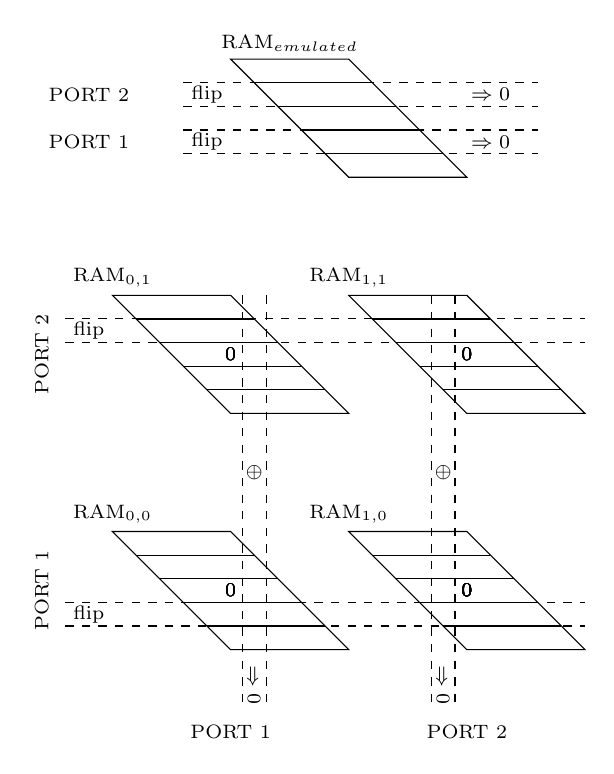
\begin{tikzpicture}[scale=3]
            \scriptsize
            \draw[] (.5,2-.25) -- (1,2-.25) -- (.5,2.25) -- (0, 2.25) -- cycle;
            \foreach \j in {-.15,-.05, .05, .15}{
                \draw[] (.25-\j, 2+\j) -- (.75-\j,2+\j);
            }
            \foreach \i/\v in {0/0,1/0,2/0,3/0,4/0}{
                \FPeval{\x}{.7-\i*.1};
                \FPeval{\y}{2-.2+\i*.1};
                \node[] at (\x,\y) {\v};
            }
            \node at (.25,2.25)[anchor=south]{RAM$_{emulated}$};
            \foreach \xram in {0,1}{
                \node at (\xram-.5,.25) [anchor=south]{RAM$_{\xram,0}$};
                \draw[xshift=\xram cm] (0,-.25) -- (.5,-.25) -- (0,.25) -- (-.5, .25) -- cycle;
                \foreach \j in {-.15,-.05, .05, .15}{
                    \draw[xshift=\xram cm] (-.25-\j, \j) -- (.25-\j,\j);
                }
                \def\y{0};
                \foreach \i/\v in {0/0,1/0,2/0,3/0,4/0}{
                    \FPeval{\x}{.2-\i*.1};
                    \FPeval{\y}{0-.2+\i*.1};
                    \node[] at (\x+\xram,\y) {\v};
                }
            }
            \foreach \xram in {0,1}{
                \node at (\xram-.5,1.25) [anchor=south]{RAM$_{\xram,1}$};
                \draw[xshift=\xram cm,yshift=1cm] (0,-.25) -- (.5,-.25) -- (0,.25) -- (-.5, .25) -- cycle;
                \foreach \j in {-.15,-.05, .05, .15}{
                    \draw[xshift=\xram cm,yshift=1cm] (-.25-\j, \j) -- (.25-\j,\j);
                }
                \def\y{0};
                \foreach \i/\v in {0/0,1/0,2/0,3/0,4/0}{
                    \FPeval{\x}{.2-\i*.1};
                    \FPeval{\y}{0-.2+\i*.1};
                    \node[] at (\x+\xram,\y+1) {\v};
                }
            }
            \node at (-.8,0)[rotate=90]{PORT 1};
            \node at (-.8,1)[rotate=90]{PORT 2};
            \node at (0,-.6){PORT 1};
            \node at (1,-.6){PORT 2};
            %TODO first and second
            \def\first{1};
            \ifthenelse{\first>0}{
            \draw[dashed] (-.7,0-.25+\first*.1) -- (1.5,0-.25+\first*.1);
            \draw[dashed] (-.7,0-.15+\first*.1) -- (1.5,0-.15+\first*.1);
            \draw[dashed] (0+.25-\first*.1,1.25) -- (0+.25-\first*.1,-.5);
            \draw[dashed] (0+.15-\first*.1,1.25) -- (0+.15-\first*.1,-.5);
            \node[rotate=270] at (0.2-\first*.1,-.4) {$\Rightarrow0$};
            \node at (0.2-\first*.1,.5) {$\oplus$};
            \node at (-.6,-.2+\first*.1) {flip};
        }{}
            \def\second{3};
            \ifthenelse{\second>0}{
            \draw[dashed] (-.7,1-.25+\second*.1) -- (1.5,1-.25+\second*.1);
            \draw[dashed] (-.7,1-.15+\second*.1) -- (1.5,1-.15+\second*.1);
            \draw[dashed] (1+.25-\second*.1,1.25) -- (1+.25-\second*.1,-.5);
            \draw[dashed] (1+.15-\second*.1,1.25) -- (1+.15-\second*.1,-.5);
            \node[rotate=270] at (1.2-\second*.1,-.4) {$\Rightarrow0$};
            \node at (1.2-\second*.1,.5) {$\oplus$};
            \node at (-.6,.8+\second*.1) {flip};
        }{}
            \ifthenelse{\first>0}{
            \draw[dashed] (-.2,2-.25+\first*.1) -- (1.3,2-.25+\first*.1);
            \draw[dashed] (-.2,2-.15+\first*.1) -- (1.3,2-.15+\first*.1);
            \node at (-.6,2-.2+\first*.1) {PORT 1};
            \node at (-.1,2-.2+\first*.1) {flip};
            \node at (1.1,2-.2+\first*.1) {$\Rightarrow0$};

        }{}
            \ifthenelse{\second>0}{
            \draw[dashed] (-.2,2-.25+\second*.1) -- (1.3,2-.25+\second*.1);
            \draw[dashed] (-.2,2-.15+\second*.1) -- (1.3,2-.15+\second*.1);
            \node at (-.6,2-.2+\second*.1) {PORT 2};
            \node at (-.1,2-.2+\second*.1) {flip};
            \node at (1.1,2-.2+\second*.1) {$\Rightarrow0$};
        }{}

        \end{tikzpicture}
        \caption{On the first clock cycle, Port 1 receives a request for cell 1 and Port 2 receives a request for cell 3.}
        \label{fig:xorram0}
    \end{subfigure}
    \begin{subfigure}{.5\linewidth}
        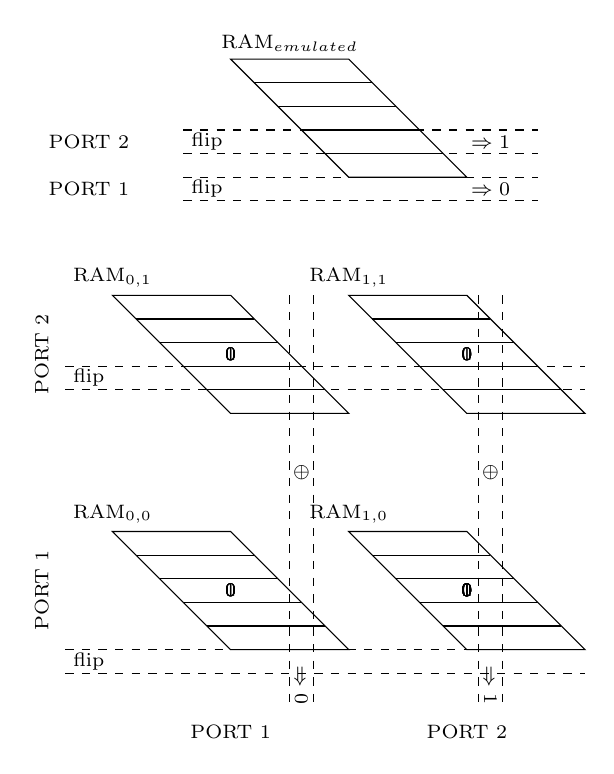
\begin{tikzpicture}[scale=3]
            \scriptsize
            \draw[] (.5,2-.25) -- (1,2-.25) -- (.5,2.25) -- (0, 2.25) -- cycle;
            \foreach \j in {-.15,-.05, .05, .15}{
                \draw[] (.25-\j, 2+\j) -- (.75-\j,2+\j);
            }
            \foreach \i/\v in {0/0,1/1,2/0,3/1,4/0}{
                \FPeval{\x}{.7-\i*.1};
                \FPeval{\y}{2-.2+\i*.1};
                \node[] at (\x,\y) {\v};
            }
            \node at (.25,2.25)[anchor=south]{RAM$_{emulated}$};
            \foreach \xram in {0,1}{
                \node at (\xram-.5,.25) [anchor=south]{RAM$_{\xram,0}$};
                \draw[xshift=\xram cm] (0,-.25) -- (.5,-.25) -- (0,.25) -- (-.5, .25) -- cycle;
                \foreach \j in {-.15,-.05, .05, .15}{
                    \draw[xshift=\xram cm] (-.25-\j, \j) -- (.25-\j,\j);
                }
                \def\y{0};
                \foreach \i/\v in {0/0,1/1,2/0,3/0,4/0}{
                    \FPeval{\x}{.2-\i*.1};
                    \FPeval{\y}{0-.2+\i*.1};
                    \node[] at (\x+\xram,\y) {\v};
                }
            }
            \foreach \xram in {0,1}{
                \node at (\xram-.5,1.25) [anchor=south]{RAM$_{\xram,1}$};
                \draw[xshift=\xram cm,yshift=1cm] (0,-.25) -- (.5,-.25) -- (0,.25) -- (-.5, .25) -- cycle;
                \foreach \j in {-.15,-.05, .05, .15}{
                    \draw[xshift=\xram cm,yshift=1cm] (-.25-\j, \j) -- (.25-\j,\j);
                }
                \def\y{0};
                \foreach \i/\v in {0/0,1/0,2/0,3/1,4/0}{
                    \FPeval{\x}{.2-\i*.1};
                    \FPeval{\y}{0-.2+\i*.1};
                    \node[] at (\x+\xram,\y+1) {\v};
                }
            }
            \node at (-.8,0)[rotate=90]{PORT 1};
            \node at (-.8,1)[rotate=90]{PORT 2};
            \node at (0,-.6){PORT 1};
            \node at (1,-.6){PORT 2};
            %TODO first and second
            \def\first{-1};
            \ifthenelse{\first>0}{
            \draw[dashed] (-.7,0-.25+\first*.1) -- (1.5,0-.25+\first*.1);
            \draw[dashed] (-.7,0-.15+\first*.1) -- (1.5,0-.15+\first*.1);
            \draw[dashed] (0+.25-\first*.1,1.25) -- (0+.25-\first*.1,-.5);
            \draw[dashed] (0+.15-\first*.1,1.25) -- (0+.15-\first*.1,-.5);
            \node[rotate=270] at (0.2-\first*.1,-.4) {$\Rightarrow 0$};
            \node at (0.2-\first*.1,.5) {$\oplus$};
            \node at (-.6,-.2+\first*.1) {flip};
        }{}
            \def\second{1};
            \ifthenelse{\second>0}{
            \draw[dashed] (-.7,1-.25+\second*.1) -- (1.5,1-.25+\second*.1);
            \draw[dashed] (-.7,1-.15+\second*.1) -- (1.5,1-.15+\second*.1);
            \draw[dashed] (1+.25-\second*.1,1.25) -- (1+.25-\second*.1,-.5);
            \draw[dashed] (1+.15-\second*.1,1.25) -- (1+.15-\second*.1,-.5);
            \node[rotate=270] at (1.2-\second*.1,-.4) {$\Rightarrow 1$};
            \node at (1.2-\second*.1,.5) {$\oplus$};
            \node at (-.6,.8+\second*.1) {flip};
        }{}
            \ifthenelse{\first>0}{
            \draw[dashed] (-.2,2-.25+\first*.1) -- (1.3,2-.25+\first*.1);
            \draw[dashed] (-.2,2-.15+\first*.1) -- (1.3,2-.15+\first*.1);
            \node at (-.6,2-.2+\first*.1) {PORT 1};
            \node at (-.1,2-.2+\first*.1) {flip};
            \node at (1.1,2-.2+\first*.1) {$\Rightarrow 0$};

        }{}
            \ifthenelse{\second>0}{
            \draw[dashed] (-.2,2-.25+\second*.1) -- (1.3,2-.25+\second*.1);
            \draw[dashed] (-.2,2-.15+\second*.1) -- (1.3,2-.15+\second*.1);
            \node at (-.6,2-.2+\second*.1) {PORT 2};
            \node at (-.1,2-.2+\second*.1) {flip};
            \node at (1.1,2-.2+\second*.1) {$\Rightarrow 1$};
        }{}

        \end{tikzpicture}
        \caption{On the second clock cycle, Port 2 receives a request for cell 1 and Port 1 does not receive a request.}
        \label{fig:xorram1}
    \end{subfigure}
    \begin{subfigure}{.5\linewidth}
        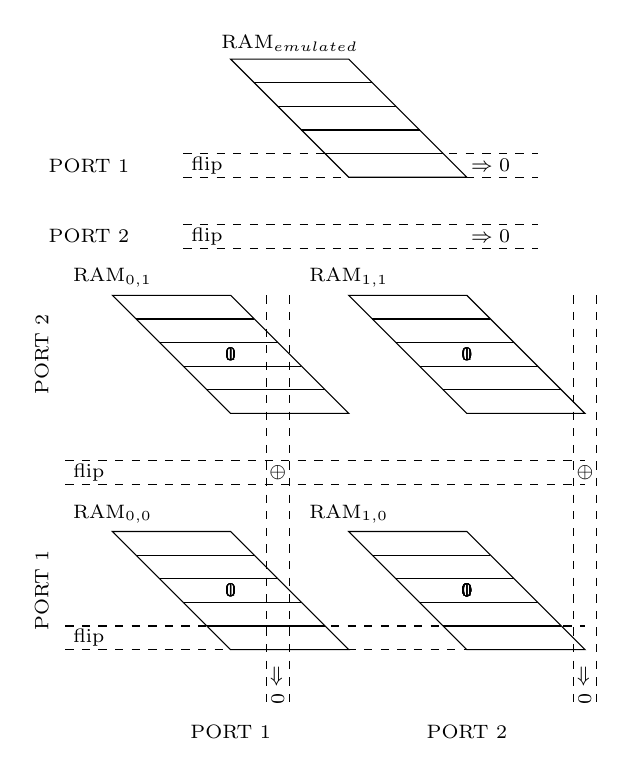
\begin{tikzpicture}[scale=3]
            \scriptsize
            \draw[] (.5,2-.25) -- (1,2-.25) -- (.5,2.25) -- (0, 2.25) -- cycle;
            \foreach \j in {-.15,-.05, .05, .15}{
                \draw[] (.25-\j, 2+\j) -- (.75-\j,2+\j);
            }
            \foreach \i/\v in {0/0,1/0,2/0,3/1,4/0}{
                \FPeval{\x}{.7-\i*.1};
                \FPeval{\y}{2-.2+\i*.1};
                \node[] at (\x,\y) {\v};
            }
            \node at (.25,2.25)[anchor=south]{RAM$_{emulated}$};
            \foreach \xram in {0,1}{
                \node at (\xram-.5,.25) [anchor=south]{RAM$_{\xram,0}$};
                \draw[xshift=\xram cm] (0,-.25) -- (.5,-.25) -- (0,.25) -- (-.5, .25) -- cycle;
                \foreach \j in {-.15,-.05, .05, .15}{
                    \draw[xshift=\xram cm] (-.25-\j, \j) -- (.25-\j,\j);
                }
                \def\y{0};
                \foreach \i/\v in {0/0,1/1,2/0,3/0,4/0}{
                    \FPeval{\x}{.2-\i*.1};
                    \FPeval{\y}{0-.2+\i*.1};
                    \node[] at (\x+\xram,\y) {\v};
                }
            }
            \foreach \xram in {0,1}{
                \node at (\xram-.5,1.25) [anchor=south]{RAM$_{\xram,1}$};
                \draw[xshift=\xram cm,yshift=1cm] (0,-.25) -- (.5,-.25) -- (0,.25) -- (-.5, .25) -- cycle;
                \foreach \j in {-.15,-.05, .05, .15}{
                    \draw[xshift=\xram cm,yshift=1cm] (-.25-\j, \j) -- (.25-\j,\j);
                }
                \def\y{0};
                \foreach \i/\v in {0/0,1/1,2/0,3/1,4/0}{
                    \FPeval{\x}{.2-\i*.1};
                    \FPeval{\y}{0-.2+\i*.1};
                    \node[] at (\x+\xram,\y+1) {\v};
                }
            }
            \node at (-.8,0)[rotate=90]{PORT 1};
            \node at (-.8,1)[rotate=90]{PORT 2};
            \node at (0,-.6){PORT 1};
            \node at (1,-.6){PORT 2};
            %TODO first and second
            \def\first{0};
            \ifthenelse{\first>-1}{
            \draw[dashed] (-.7,0-.25+\first*.1) -- (1.5,0-.25+\first*.1);
            \draw[dashed] (-.7,0-.15+\first*.1) -- (1.5,0-.15+\first*.1);
            \draw[dashed] (0+.25-\first*.1,1.25) -- (0+.25-\first*.1,-.5);
            \draw[dashed] (0+.15-\first*.1,1.25) -- (0+.15-\first*.1,-.5);
            \node[rotate=270] at (0.2-\first*.1,-.4) {$\Rightarrow 0$};
            \node at (0.2-\first*.1,.5) {$\oplus$};
            \node at (-.6,-.2+\first*.1) {flip};
        }{}
            \def\second{-3};
            \ifthenelse{\second>0}{
            \draw[dashed] (-.7,1-.25+\second*.1) -- (1.5,1-.25+\second*.1);
            \draw[dashed] (-.7,1-.15+\second*.1) -- (1.5,1-.15+\second*.1);
            \draw[dashed] (1+.25-\second*.1,1.25) -- (1+.25-\second*.1,-.5);
            \draw[dashed] (1+.15-\second*.1,1.25) -- (1+.15-\second*.1,-.5);
            \node[rotate=270] at (1.2-\second*.1,-.4) {$\Rightarrow 0$};
            \node at (1.2-\second*.1,.5) {$\oplus$};
            \node at (-.6,.8+\second*.1) {flip};
        }{}
            \ifthenelse{\first>-1}{
            \draw[dashed] (-.2,2-.25+\first*.1) -- (1.3,2-.25+\first*.1);
            \draw[dashed] (-.2,2-.15+\first*.1) -- (1.3,2-.15+\first*.1);
            \node at (-.6,2-.2+\first*.1) {PORT 1};
            \node at (-.1,2-.2+\first*.1) {flip};
            \node at (1.1,2-.2+\first*.1) {$\Rightarrow 0$};

        }{}
            \ifthenelse{\second>0}{
            \draw[dashed] (-.2,2-.25+\second*.1) -- (1.3,2-.25+\second*.1);
            \draw[dashed] (-.2,2-.15+\second*.1) -- (1.3,2-.15+\second*.1);
            \node at (-.6,2-.2+\second*.1) {PORT 2};
            \node at (-.1,2-.2+\second*.1) {flip};
            \node at (1.1,2-.2+\second*.1) {$\Rightarrow 0$};
        }{}

        \end{tikzpicture}
        \caption{On the third clock cycle, Port 1 receives a request for cell 0 and Port 2 does not receive a request.}
        \label{fig:xorram2}
    \end{subfigure}
    \begin{subfigure}{.5\linewidth}
        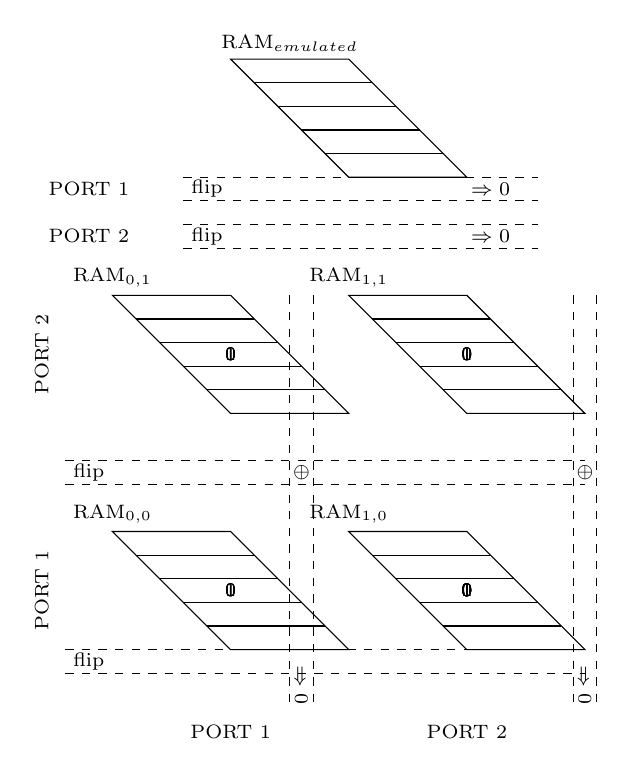
\begin{tikzpicture}[scale=3]
            \scriptsize
            \draw[] (.5,2-.25) -- (1,2-.25) -- (.5,2.25) -- (0, 2.25) -- cycle;
            \foreach \j in {-.15,-.05, .05, .15}{
                \draw[] (.25-\j, 2+\j) -- (.75-\j,2+\j);
            }
            \foreach \i/\v in {0/1,1/0,2/0,3/1,4/0}{
                \FPeval{\x}{.7-\i*.1};
                \FPeval{\y}{2-.2+\i*.1};
                \node[] at (\x,\y) {\v};
            }
            \node at (.25,2.25)[anchor=south]{RAM$_{emulated}$};
            \foreach \xram in {0,1}{
                \node at (\xram-.5,.25) [anchor=south]{RAM$_{\xram,0}$};
                \draw[xshift=\xram cm] (0,-.25) -- (.5,-.25) -- (0,.25) -- (-.5, .25) -- cycle;
                \foreach \j in {-.15,-.05, .05, .15}{
                    \draw[xshift=\xram cm] (-.25-\j, \j) -- (.25-\j,\j);
                }
                \def\y{0};
                \foreach \i/\v in {0/1,1/1,2/0,3/0,4/0}{
                    \FPeval{\x}{.2-\i*.1};
                    \FPeval{\y}{0-.2+\i*.1};
                    \node[] at (\x+\xram,\y) {\v};
                }
            }
            \foreach \xram in {0,1}{
                \node at (\xram-.5,1.25) [anchor=south]{RAM$_{\xram,1}$};
                \draw[xshift=\xram cm,yshift=1cm] (0,-.25) -- (.5,-.25) -- (0,.25) -- (-.5, .25) -- cycle;
                \foreach \j in {-.15,-.05, .05, .15}{
                    \draw[xshift=\xram cm,yshift=1cm] (-.25-\j, \j) -- (.25-\j,\j);
                }
                \def\y{0};
                \foreach \i/\v in {0/0,1/1,2/0,3/1,4/0}{
                    \FPeval{\x}{.2-\i*.1};
                    \FPeval{\y}{0-.2+\i*.1};
                    \node[] at (\x+\xram,\y+1) {\v};
                }
            }
            \node at (-.8,0)[rotate=90]{PORT 1};
            \node at (-.8,1)[rotate=90]{PORT 2};
            \node at (0,-.6){PORT 1};
            \node at (1,-.6){PORT 2};
            %TODO first and second
            \def\first{-1};
            \ifthenelse{\first>0}{
            \draw[dashed] (-.7,0-.25+\first*.1) -- (1.5,0-.25+\first*.1);
            \draw[dashed] (-.7,0-.15+\first*.1) -- (1.5,0-.15+\first*.1);
            \draw[dashed] (0+.25-\first*.1,1.25) -- (0+.25-\first*.1,-.5);
            \draw[dashed] (0+.15-\first*.1,1.25) -- (0+.15-\first*.1,-.5);
            \node[rotate=270] at (0.2-\first*.1,-.4) {$\Rightarrow 0$};
            \node at (0.2-\first*.1,.5) {$\oplus$};
            \node at (-.6,-.2+\first*.1) {flip};
        }{}
            \def\second{-3};
            \ifthenelse{\second>0}{
            \draw[dashed] (-.7,1-.25+\second*.1) -- (1.5,1-.25+\second*.1);
            \draw[dashed] (-.7,1-.15+\second*.1) -- (1.5,1-.15+\second*.1);
            \draw[dashed] (1+.25-\second*.1,1.25) -- (1+.25-\second*.1,-.5);
            \draw[dashed] (1+.15-\second*.1,1.25) -- (1+.15-\second*.1,-.5);
            \node[rotate=270] at (1.2-\second*.1,-.4) {$\Rightarrow 0$};
            \node at (1.2-\second*.1,.5) {$\oplus$};
            \node at (-.6,.8+\second*.1) {flip};
        }{}
            \ifthenelse{\first>0}{
            \draw[dashed] (-.2,2-.25+\first*.1) -- (1.3,2-.25+\first*.1);
            \draw[dashed] (-.2,2-.15+\first*.1) -- (1.3,2-.15+\first*.1);
            \node at (-.6,2-.2+\first*.1) {PORT 1};
            \node at (-.1,2-.2+\first*.1) {flip};
            \node at (1.1,2-.2+\first*.1) {$\Rightarrow 0$};

        }{}
            \ifthenelse{\second>0}{
            \draw[dashed] (-.2,2-.25+\second*.1) -- (1.3,2-.25+\second*.1);
            \draw[dashed] (-.2,2-.15+\second*.1) -- (1.3,2-.15+\second*.1);
            \node at (-.6,2-.2+\second*.1) {PORT 2};
            \node at (-.1,2-.2+\second*.1) {flip};
            \node at (1.1,2-.2+\second*.1) {$\Rightarrow 0$};
        }{}

        \end{tikzpicture}
        \caption{On the fourth clock cycle, neither Port 1 or Port 2 receives a request.}
        \label{fig:xorram3}
    \end{subfigure}
    \caption[Dual port RAM with zero clock cycle read latency]{This example shows 4 clock cycles of operation of a $1\times 5$ dual port RAM, created by combining 4 pseudo dual-port RAMs.}
    \label{fig:xorram}
\end{figure}
